\chapter{\noun{Use cases}   }
In his chapter we present sequence diagram of the actions performed in the range of Pharmacy Module. Each step is detailed described. Not all actions are strongly required - sometimes it should depend on the security level requirement and budget possibilities. 

The first step is communication initialization. Actions performed in this step by the system elements are presented on the figure \ref{fig:s_q_step_1}
\begin{figure}	
	\hspace*{-1.5in}
    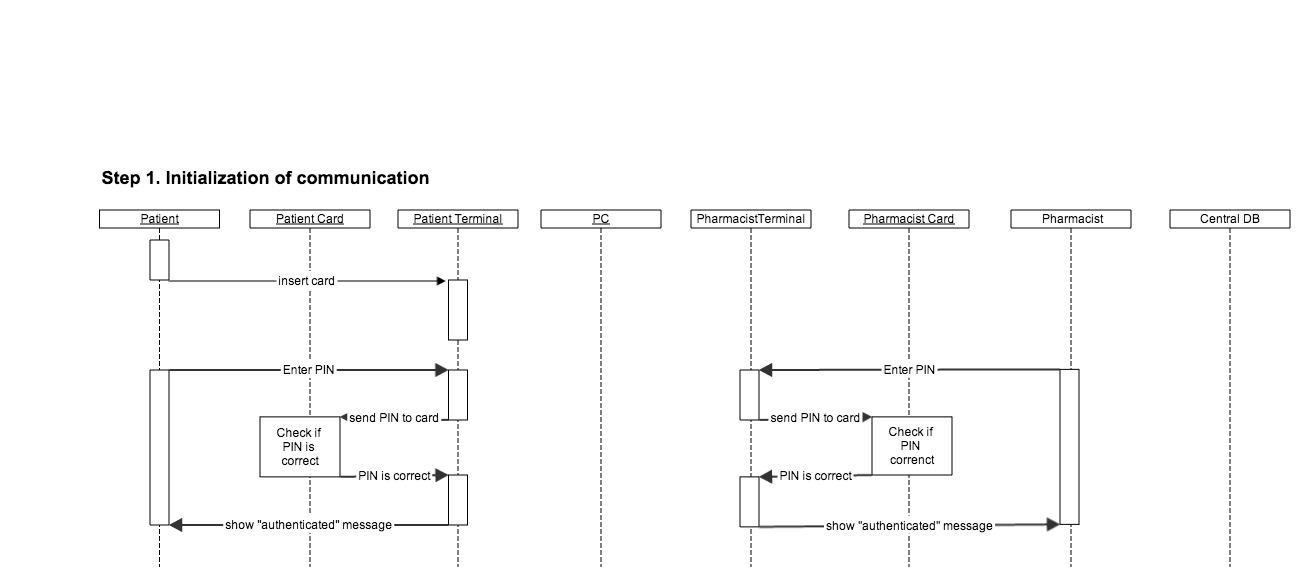
\includegraphics[scale=0.45]{s_d_1.png}
    \caption{Sequence diagram - step 1}
    \label{fig:s_q_step_1}
\end{figure} 

At the beginning, the patient put his personal card to the terminal and he enter the PIN as usual e.g. in the ATM. If the PIN is correct, the user can show appropriate message on the terminal screen. Also the pharmacist have to use his card and enter the PIN in the second terminal. Then, the system is ready to work. 

Necessity to use the PIN by the user and the pharmacist prevents the risk the situation, when e.g. the card was stolen or lost.


\begin{figure}	
	\hspace*{-1.5in}
    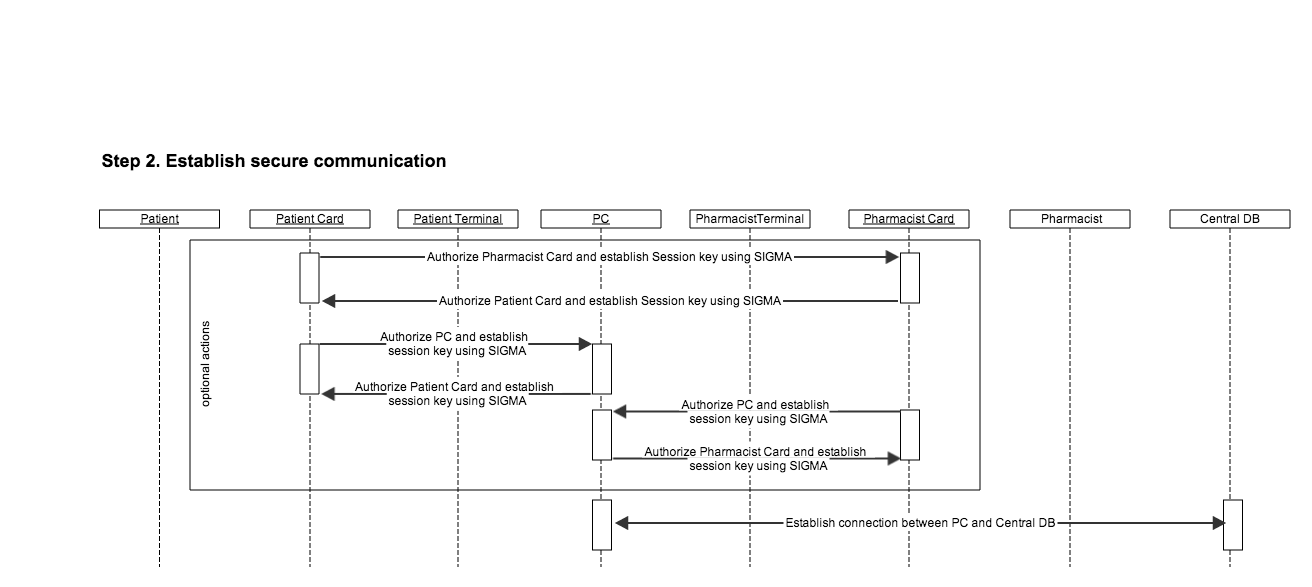
\includegraphics[scale=0.45]{s_d_2.png}
    \caption{Sequence diagram - step 2}
    \label{fig:s_q_step_2}
\end{figure} 

The second step, presented on the figure \ref{fig:s_q_step_2}, contains actions related with establishing secure communication ways between the system parties. There are marked the actions, which are optional and are not required for the system to work properly. Establishing secure communication between the cards allows the participant to be sure, that the patient ant pharmacist cards are not the fake cards and they are authenticated to each other.
Similarly, suing the SIGMA protocol between the card (patient or pharmacist) and the application installed on the PC, allows to authorization the application by the card and the card by the application. However. this two sub-steps can be implement, if the very-high level of the security from this point of view is required. 

\begin{figure}	
	\hspace*{-1.5in}
    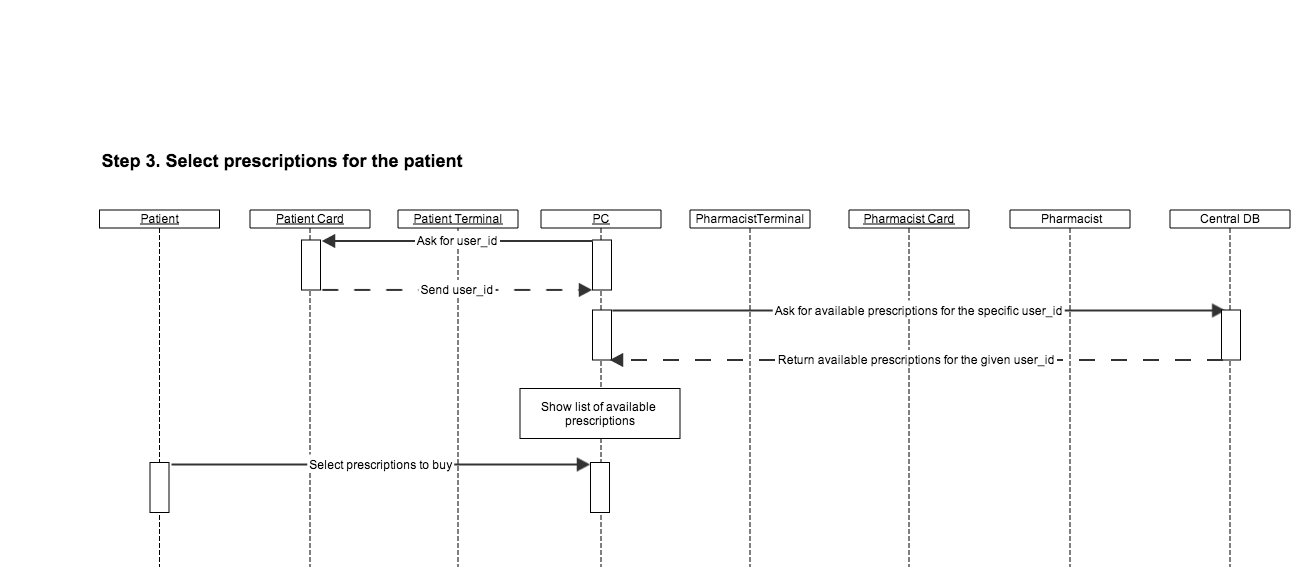
\includegraphics[scale=0.45]{s_d_3.png}
    \caption{Sequence diagram - step 3}
    \label{fig:s_q_step_3}
\end{figure} 

The figure \ref{fig:s_q_step_3} presents the point in the protocol, when the prescriptions for the user are download from the Central Database and are shown on the screen. Then, the patient have the possibility to select one or more of them to realize them. The data of the user are saved inside the patient card, so the application have to get this data to download appropriate prescriptions. 

\begin{figure}	
	\hspace*{-1.5in}
    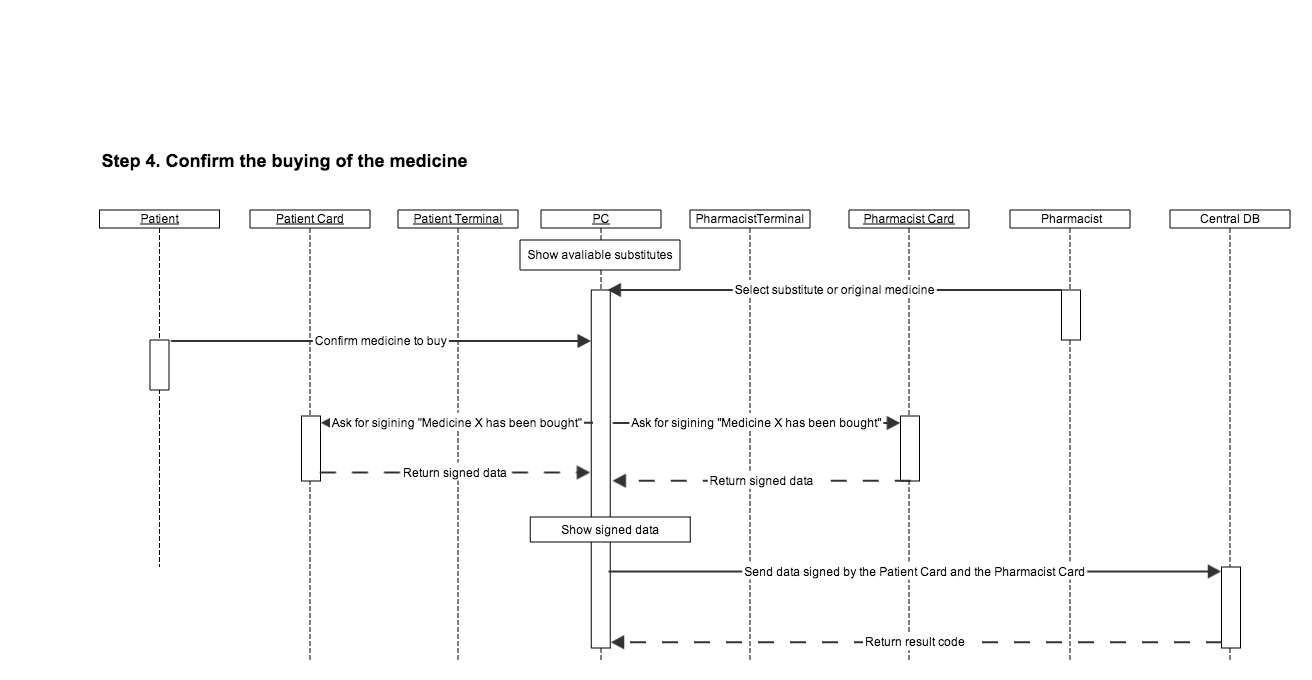
\includegraphics[scale=0.45]{s_d_4.png}
    \caption{Sequence diagram - step 4}
    \label{fig:s_q_step_4}
\end{figure} 



